\chapter{Validaci\'on y Resultados}
\label{chap:resultados}

\section{La misi\'on SAC-D}
\subsection{El modelo SGP4}
Se listan a continuaci\'on dos tablas con las efem\'erides de la misi\'on SAC-D, de los primeros cuatro minutos del d\'ia 01/01/2013.
Ambas fueron generadas a partir del mismo TLE.\\

\underline{TLE.}
\begin{verbatim}
1 37673U 11024A   13001.74853505  .00000428  00000-0  75550-4 0  9996
2 37673 098.0122 011.5654 0001526 107.5603 009.0604 14.72289948 84036
\end{verbatim}

La tabla \ref{tab:arcode} muestra los resultados que genera ARxCODE propagando con la librer\'ia SGP4 de python.
La tabla \ref{tab:stk} muestra los resultados que genera el STK a partir del modelo SGP4.\\

Salida ARxCODE.\\

\begin{tabular}{lcccccc}
2013-01-01 00:00:00&-2372.76245& -1381.01830& 6465.57494& -6.95099& -0.936313& -2.7452304\\
2013-01-01 00:01:00& -2784.64672& -1434.31269& 6287.6158& -6.77374& -0.839556& -3.1847058\\
2013-01-01 00:02:00& -3185.05363& -1481.69530& 6083.67196& -6.56854& -0.739322& -3.611093\\
2013-01-01 00:03:00& -3572.3305& -1522.96975& 5854.58154& -6.336229& -0.636021& -4.022632\\
2013-01-01 00:04:00& -3944.8780& -1557.96472& 5601.28702& -6.077737& -0.53007& -4.417616
\label{tab:arcode}
\end{tabular}

Salida STK.\\

\begin{tabular}{lcccccc}
2013-01-01 00:00:00&-2372.763028&-1381.020186&6465.574337&-6.950997&-0.936317&-2.745232\\
2013-01-01 00:01:00&-2784.647262&-1434.314738&6287.615189&-6.773748&-0.839559&-3.184707\\
2013-01-01 00:02:00&-3185.054138&-1481.697504&6083.671167&-6.568547&-0.739325&-3.611095\\
2013-01-01 00:03:00&-3572.330976&-1522.972104&5854.580649&-6.336228&-0.636024&-4.022633\\
2013-01-01 00:04:00&-3944.878498&-1557.967210&5601.286042&-6.077737&-0.530081&-4.417618
\label{tab:stk}
\end{tabular}

\section{Estabilidad en la Estimaci\'on de Errores}
Constatamos que fuera de los intervalos de maniobras por commissioning o maniobras de rutina, los TLE tiene un error que es {\it{acotado}}, {\it{estable}} y\/o modelable. Por un lado con esta demostraci\'on podemos encontrar un m\'etodo de correcci\'on en la posici\'on del desecho basada en TLE. Como para encontrarla vamos a utilizar las estimaciones basadas en las comparaciones de TLEs y datos m\'as precisos de la misi\'on primaria, que esta s\'i tiene maniobras, va a ser importante detectar intervalos de maniobras de la misión ({\it{outliers}}) para descartarlos en la estimaci\'on de errores o ajuste y modelado del comportamiento de los TLE.\\


\section*{Tendencia Anual 26/07/2011 - 26/07/2012}
\begin{figure}[!h]
\centering
  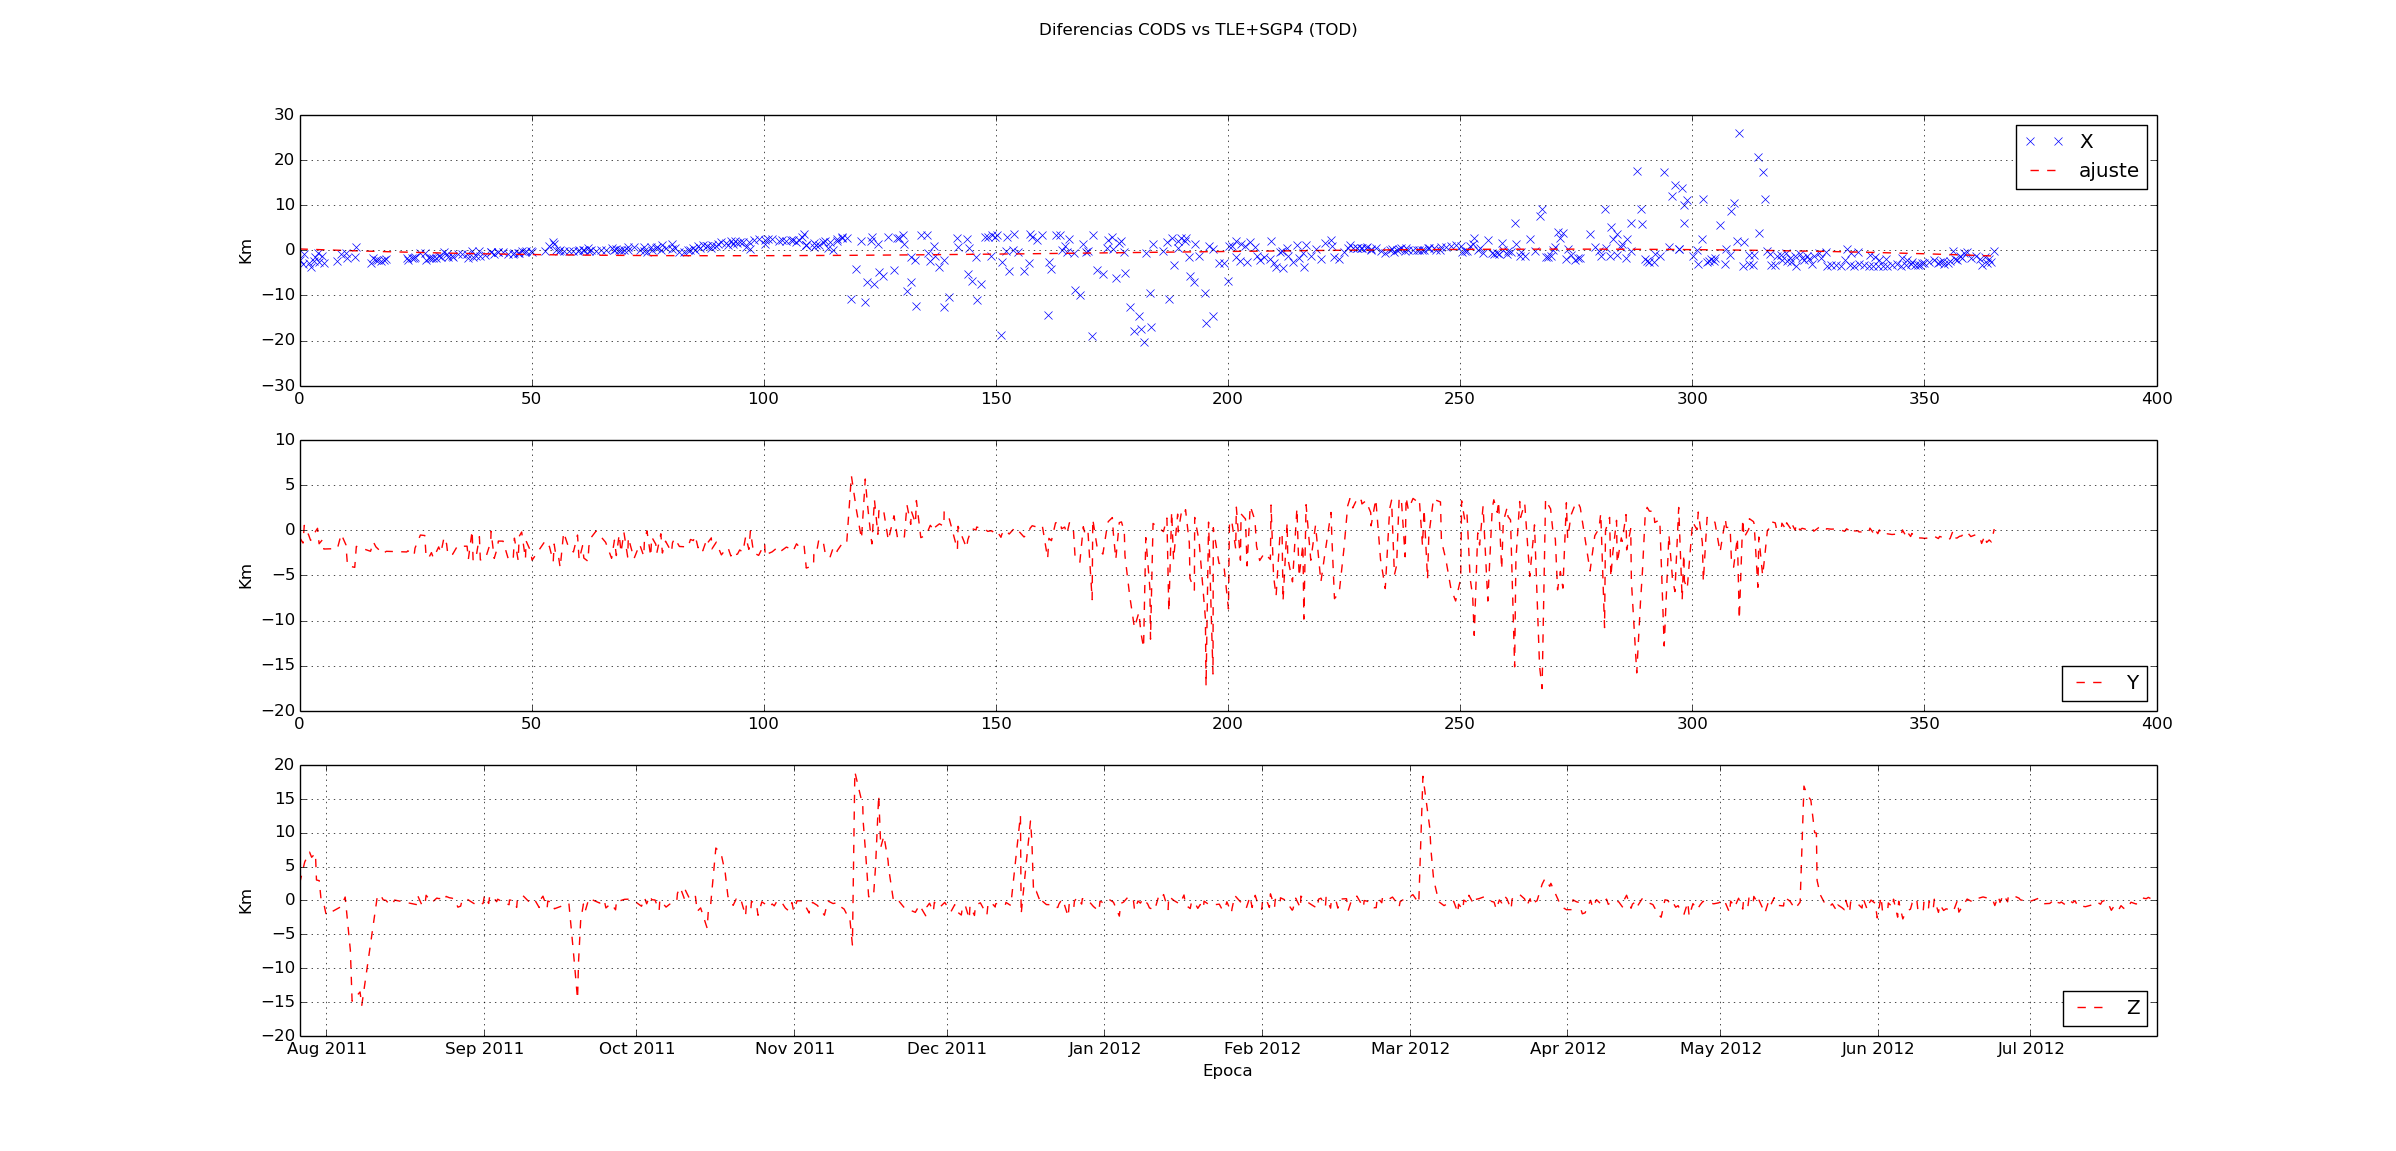
\includegraphics[width=\textwidth]{imagenes/SACD2012tod}
  \caption{Tendencia anual de las diferencias contra los datos de CODS en coordenadas X,Y,X}
\end{figure}

\section*{Tendencia Anual 01/01/2013 - 30/08/2013}
\begin{figure}[!h]
\centering
  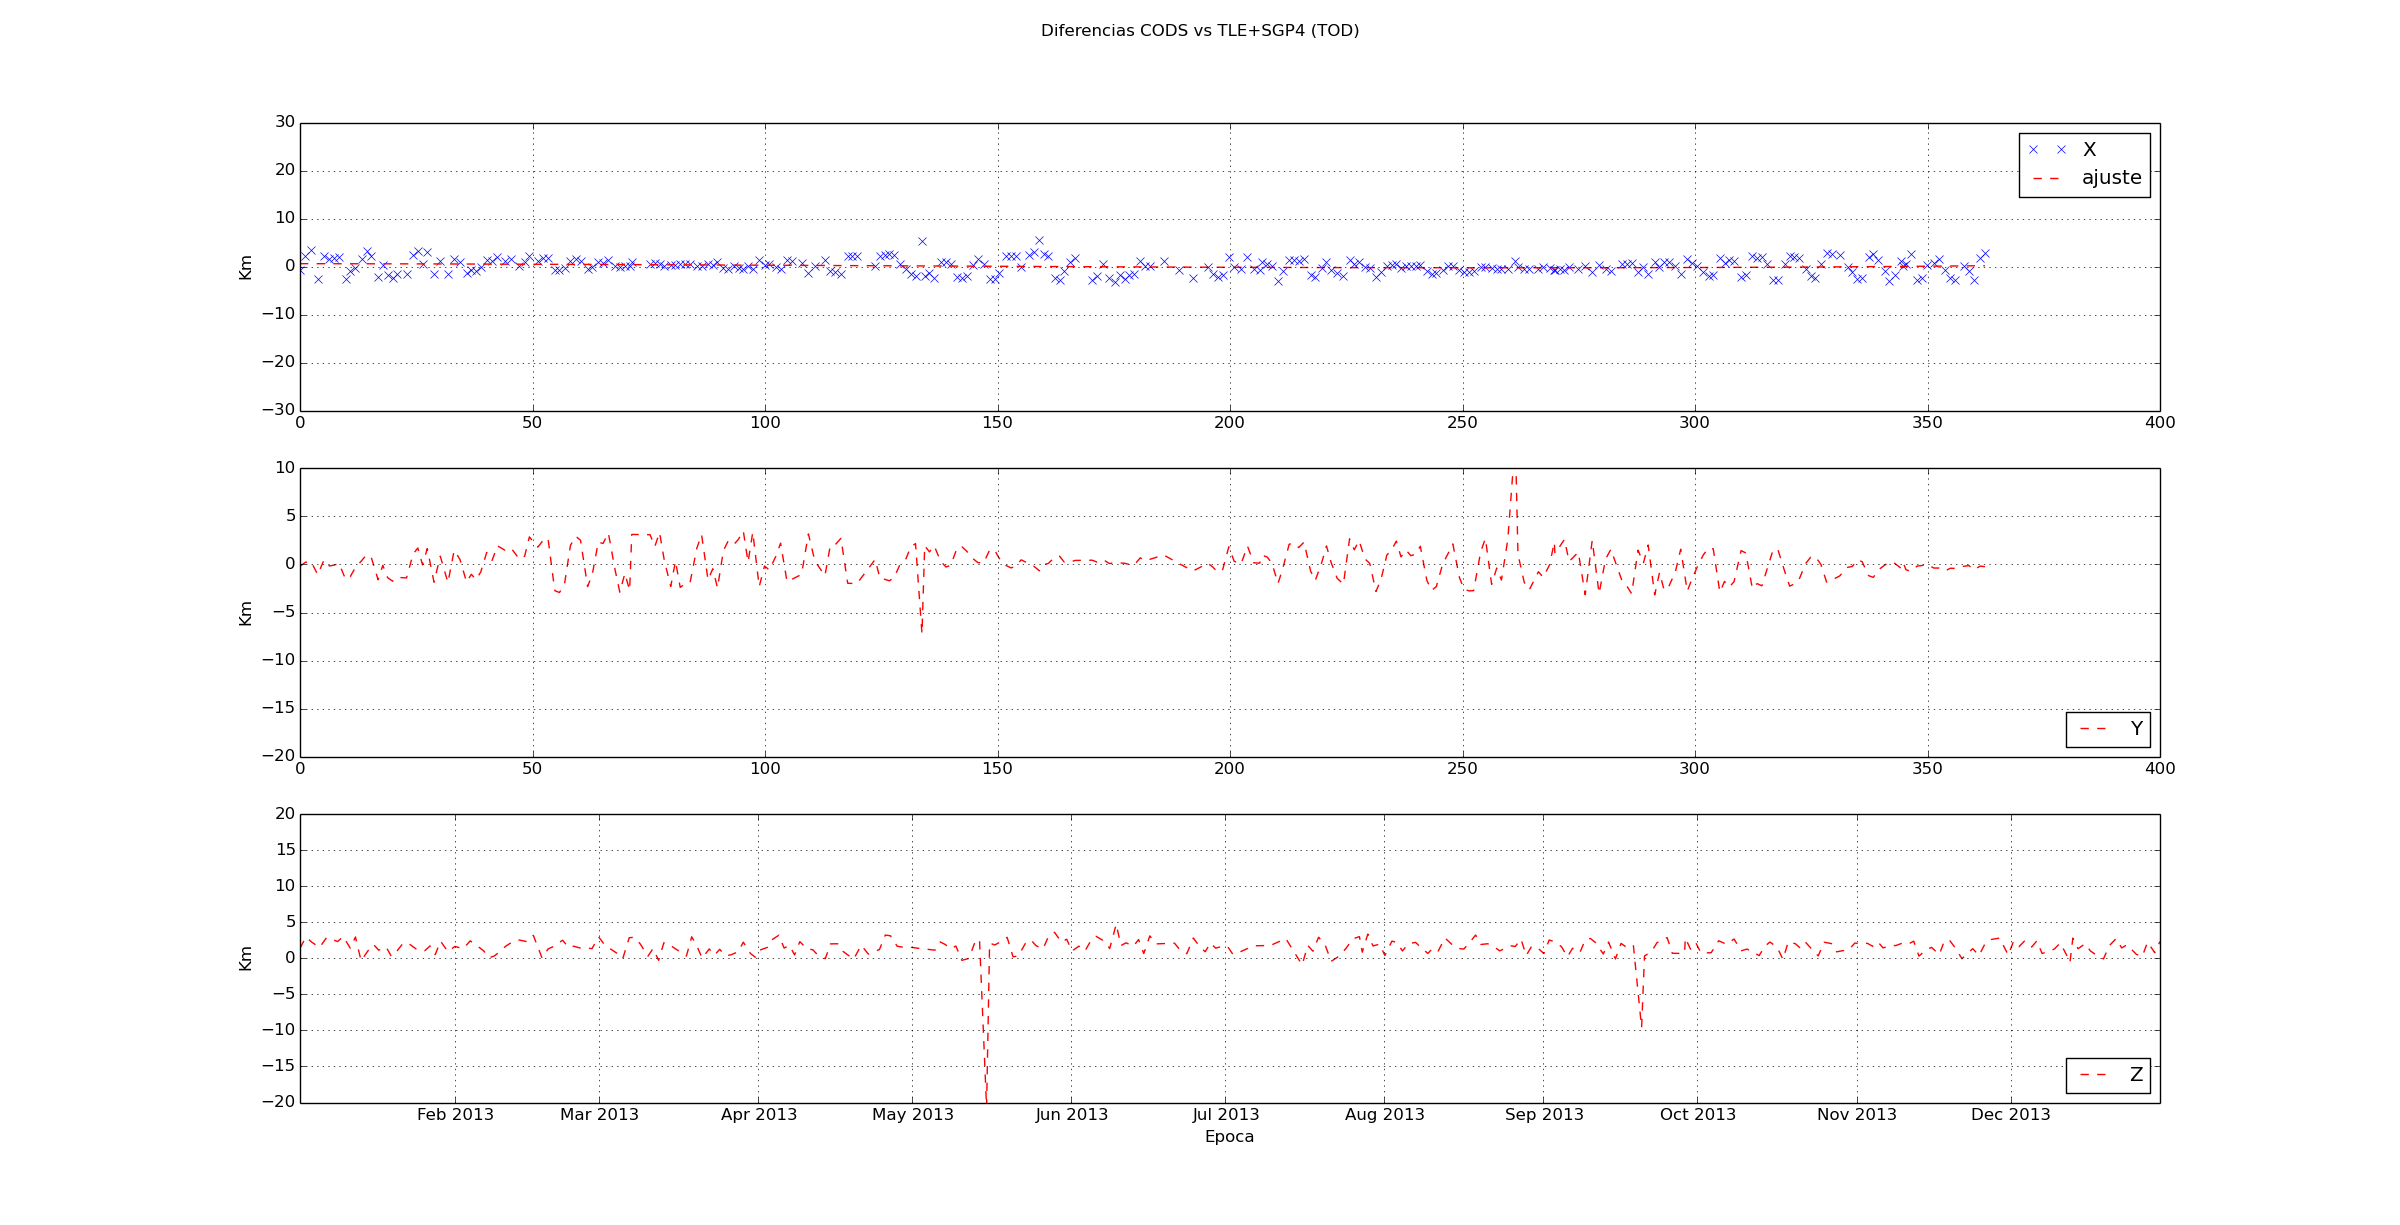
\includegraphics[width=\textwidth]{imagenes/SACD2013todEjesajustados}
  \caption{Tendencia anual de las diferencias contra los datos de CODS en coordenadas X,Y,X (descartar dia: 20/09/2013 falta de datos CODS en esa fecha)}
\end{figure}
\begin{figure}[!h]
\centering
  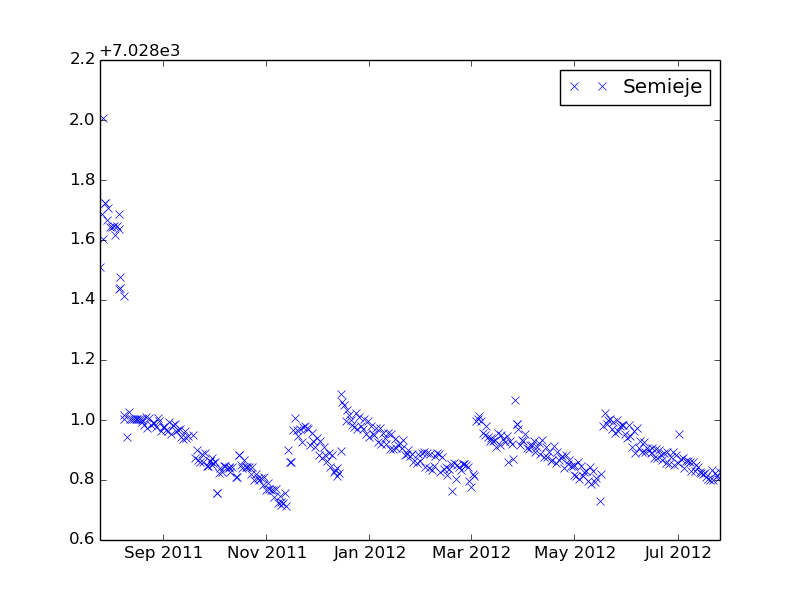
\includegraphics[width=0.7\textwidth]{imagenes/sacDtendSemi}
\end{figure}
\begin{figure}[!h]
\centering
  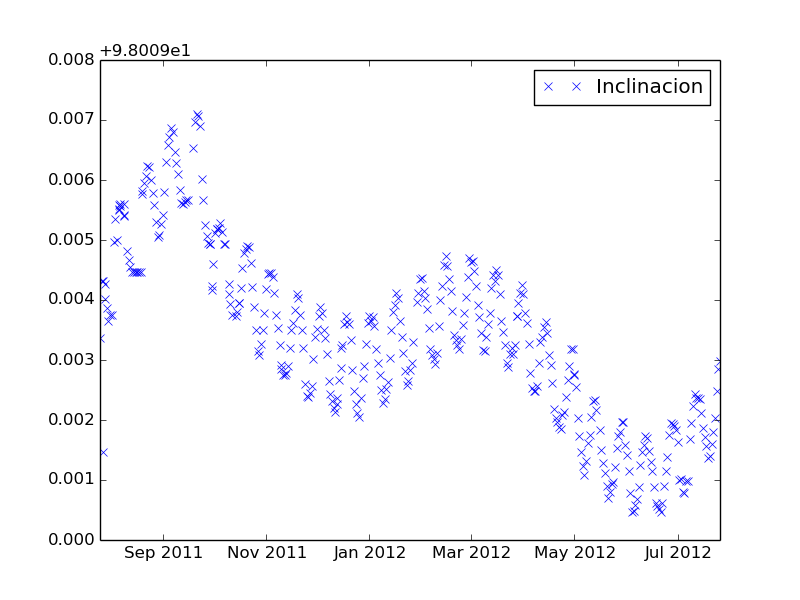
\includegraphics[width=0.7\textwidth]{imagenes/sacDtendInc}
\end{figure}


\section*{AJUSTES 26/07/2011 - 26/07/2012}
\subsection*{Lineal}
\begin{figure}[!h]
\centering
  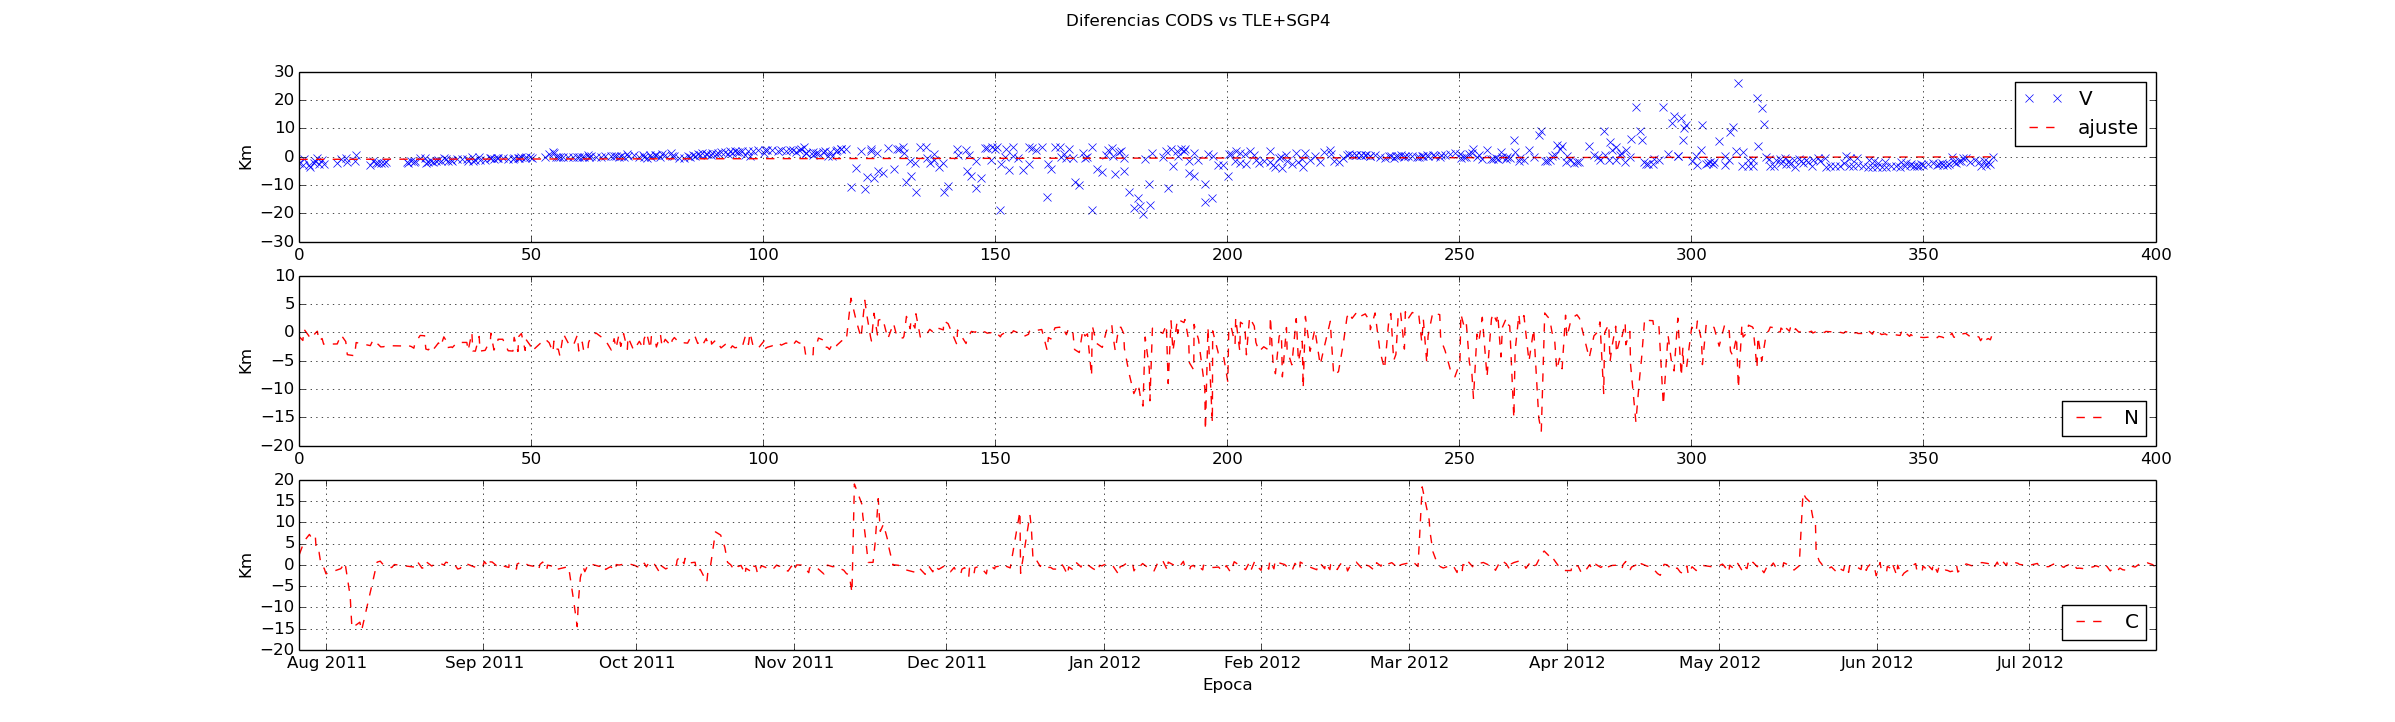
\includegraphics[width=\textwidth]{imagenes/sacDajusteG1}
\end{figure}
\begin{verbatim}
[-0.91541786  0.00237725]
[array([ 10308.58816238]), 2, array([ 1.36891754,  0.35505599])
1.2301271112846734e-13]
\end{verbatim}

\subsection*{Cuadr\'atico}
\begin{figure}[!h]
\centering
  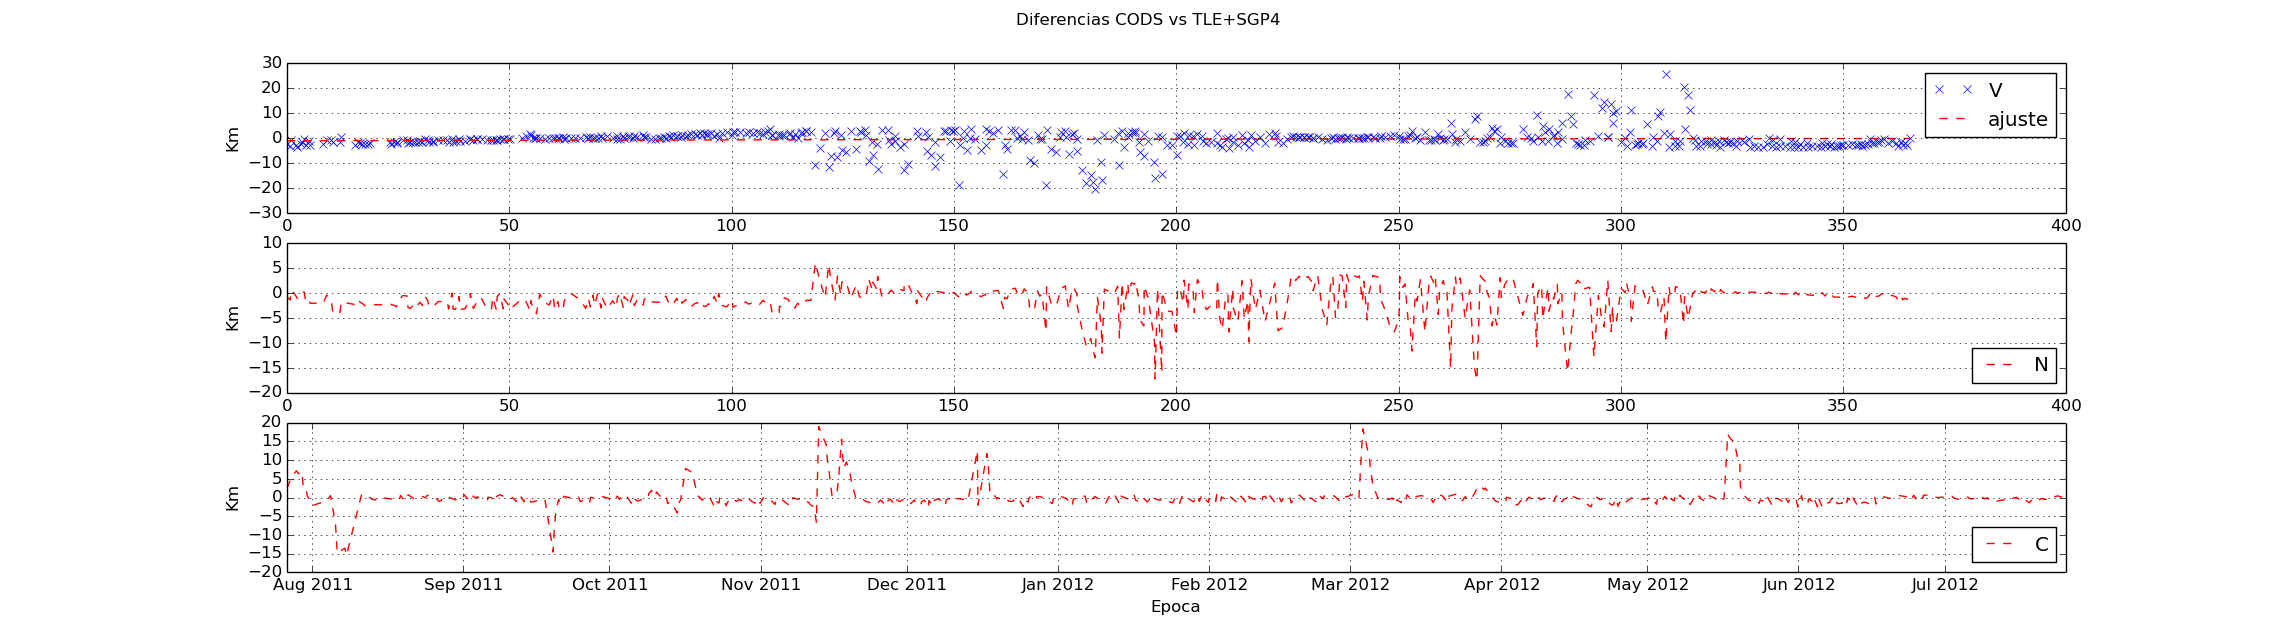
\includegraphics[width=\textwidth]{imagenes/sacDajusteG2}
\end{figure}
\begin{verbatim}
[ -9.98539126e-01   3.68651957e-03  -3.51802247e-06]
[array([ 10307.92893203]), 3, array([ 1.6541132 ,  0.5052889 ,  0.09269658])
1.2301271112846734e-13]
\end{verbatim}

\subsection*{C\'ubico}
\begin{figure}[!h]
\centering
  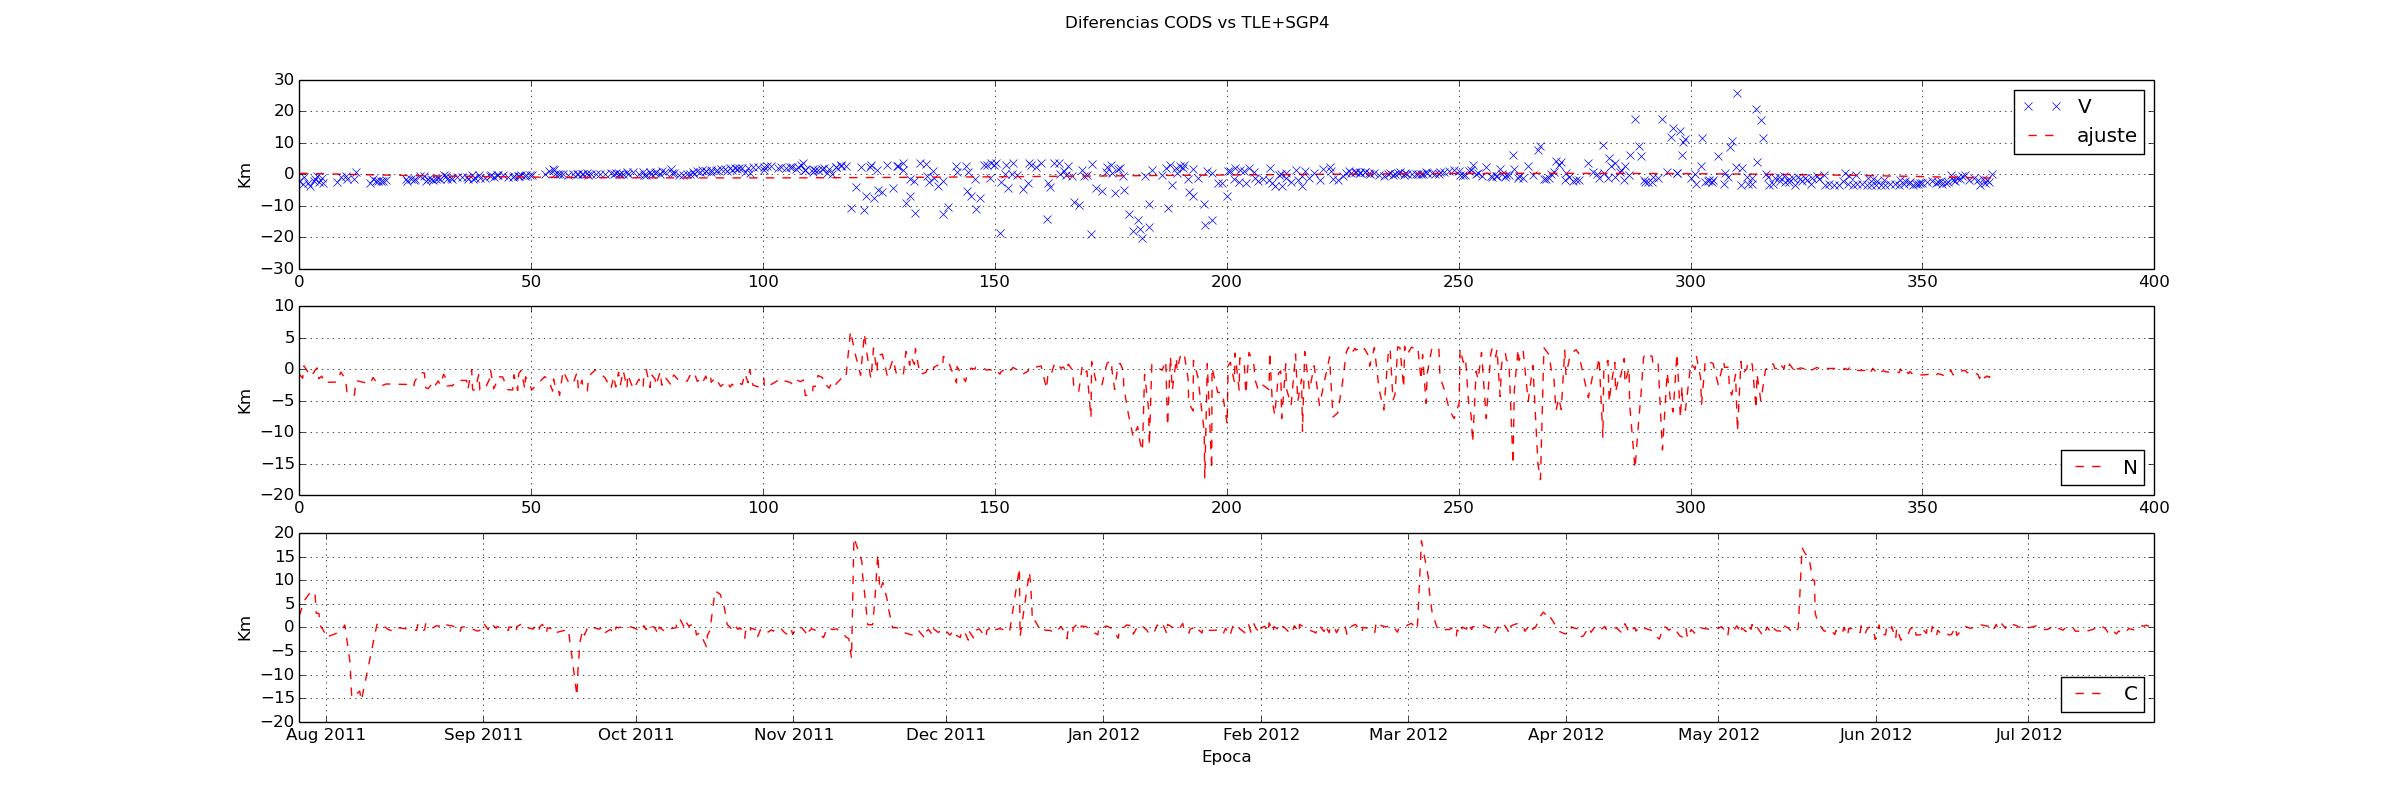
\includegraphics[width=\textwidth]{imagenes/sacDajusteG3}
\end{figure}
\begin{verbatim}
[  2.98290075e-01  -3.68802552e-02   2.69245141e-04  -4.92991794e-07]
[array([ 10194.70185149]), 4, array([ 1.89728074,  0.61374011,  0.15234123,  0.02100028])
1.2301271112846734e-13]
\end{verbatim}

\section{C\'alculo de la Probabilidad de Colisi\'on}
\begin{figure}[!h]
\centering
 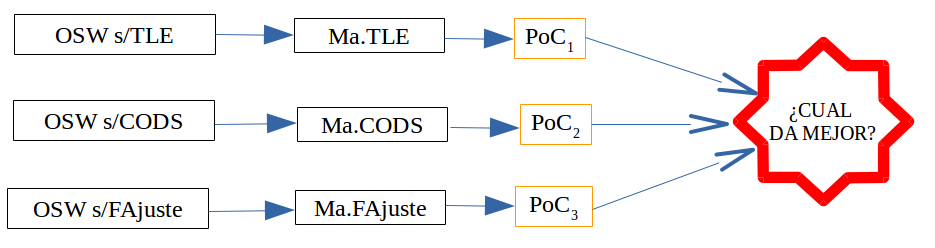
\includegraphics[width=0.5\textwidth]{imagenes/metodoARxCODE}
 \caption{Metodolog\'ia Propuesta}
 \label{fig:metodoARxCODE}
\end{figure}

